\chapter{Вглубь запроса}\label{chap:request}

Понимание внутренних процессов, зачастую, не требуется, чтобы начать
пользоваться Yesod. Однако, такое понимание часто выгодно. Эта глава проведёт
вас через процесс обработки запроса для, в общем, типичного приложения Yesod.
Обратите внимание, что изрядное количество обсуждение включает изменения кода
для версии 1.2 Yesod. Большая часть понятий совпадает с предыдущими версиями,
но используемые типы данных были слегка хаотичнее.

Yesod использует Template Haskell для генерации шаблонного кода, и это иногда
может немного усложнить понимание этого процесса. Если, помимо информации из
этой главы, вы захотите провести более глубокий анализ, может быть полезно
посмотреть код, генерируемый GHC, используя опции~\texttt{-ddump-splices}.

\begin{remark}
    Многое из представленной информации изначально было опубликовано в блоге. В
    серии, посвящённой релизу 1.2. Можете посмотреть эти публикации:

    \begin{itemize}
        \item \href{http://www.yesodweb.com/blog/2013/03/yesod-1-2-cleaner-internals}%
            {Yesod 1.2 cleaner internals}

        \item \href{http://www.yesodweb.com/blog/2013/03/big-subsite-rewrite}%
            {Big Subsite Rewrite}

        \item \href{http://www.yesodweb.com/blog/2013/03/yesod-dispatch-version-1-2}%
            {Yesod dispatch, version 1.2}
    \end{itemize}
\end{remark}

\section{Обработчики}
Пытаясь разобраться с обработкой запроса в Yesod нам необходимо рассмотреть два
процесса: как запрос перенаправляется подходящему обработчику (диспетчеризация)
и как обработчик выполняет. Начнём со второго, а затем вернёмся к
диспетчеризации.

\subsection{Слои}
Yesod построен на основе WAI, который предоставляет протокол для веб-серверов
(или, более общо, \emph{обработчиков}) и приложений для коммуникации между
собой. Для этого используется два типа данных: \lstinline'Request'
и~\lstinline'Response'. Тогда приложение (тип~\lstinline'Application')
определяется так:
\begin{lstlisting}
type Application = Request -> ResourceT IO Response
\end{lstlisting}
Обработчик WAI будет принимать приложение и выполнять его.

Типы \lstinline'Request' и \lstinline'Response' максимально возможно
низкоуровневые и пытаются представить протокол HTTP с минимумом добавлений. Это
позволяет WAI быть инструментов общего назначения, но, с другой стороны,
упускает информацию, необходимую для реализации веб-фреймворка. Например, WAI
предоставляет исходные данные для всех заголовков запроса. Но Yesod требуется
разбирать эти данные, чтобы получить информацию о куки, а затем разбирать куки,
чтобы выделить информацию о сессии.

Для работы в таких условиях Yesod вводит два новых типа данных:
\lstinline'YesodRequest' и~\lstinline'YesodResponse'. Первый содержит
тип~\lstinline'Request' WAI и также добавляет такую информацию из запроса, как
куки и переменные сессии. На стороне ответа может использовать как
тип~\lstinline'Request' WAI, так и высокоуровневое предоставление такого
ответа, включающее, например, обновлённые переменные сессии и дополнительные
заголовки ответа. По аналогии с типом~\lstinline'Application' WAI, мы вводим
тип:
\begin{lstlisting}
type YesodApp = YesodRequest -> ResourceT IO YesodResponse
\end{lstlisting}

Но, как пользователь Yesod, вы никогда, на самом деле, \lstinline'YesodApp' не
увидите. Есть ещё один уровень поверх него, предназначенный для использования
пользователями:~\lstinline'Handler'. Когда вы пишите функции-обработчики, вам
требуется доступ к следующим трём объектам:
\begin{itemize}
    \item Значение \lstinline'YesodResponse' для текущего запроса.

    \item Некоторая базовая информация из окружения, например, как
        протоколировать сообщения или как обрабатывать ошибки. Предоставляется
        типом данных~\lstinline'RunHandlerEnv'.

    \item Изменяемая переменная для отслеживания обновляемой информации,
        например, заголовков, которые надо вернуть, и состояние
        пользовательской сессии. Здесь используется~\lstinline'GHState'.

        \begin{remark}
            Имя так себе, конечно, но оно такое по историческим причинам.
        \end{remark}
\end{itemize}

Поэтому, когда вы пишите функцию-обработчик, вы, фактически, работаете в
монаде~\lstinline'Reader', имеющей доступ к описанной информации.
Функция~\lstinline'runHandler' превратит~\lstinline'Handler'
в~\lstinline'YesodApp'. Функция~\lstinline'yesodRunner' идёт ещё на шаг дальше
и превращает обработчик в~\lstinline'Application'~WAI.

\subsection{Содержимое}
Наш пример выше, как и многие другие, которые вы уже видели, демонстрирует
обработчик с типом~\lstinline'Handler Html'. Мы только что рассмотрели, что
означает~\lstinline'Handler', но откуда Yesod знает, что делать
с~\lstinline'Html'? Ответ находится в классе типов~\lstinline'ToTypedContent'.
Вот код, существенный для нашего обсуждения:
\begin{lstlisting}
data Content = ContentBuilder !BBuilder.Builder !(Maybe Int) -- ^ The content and optional content length.
             | ContentSource !(Source (ResourceT IO) (Flush BBuilder.Builder))
             | ContentFile !FilePath !(Maybe FilePart)
             | ContentDontEvaluate !Content
data TypedContent = TypedContent !ContentType !Content

class ToContent a where
    toContent :: a -> Content
class ToContent a => ToTypedContent a where
    toTypedContent :: a -> TypedContent
\end{lstlisting}

Тип данных~\lstinline'Content' описывает различные способы, которыми вы
можете предоставлять тело ответа. Первые три напрямую отражают представление
WAI. Четвёртый (\lstinline'ContentDontEvaluate') используется, чтобы указать
Yesod, что тела ответов следует полностью выполнить перед отправкой
пользователям. Преимущество полного выполнения~--- мы можем предоставлять
осмысленные сообщения об ошибках при возникновении исключения в чистом коде.
Недостатки~--- возможно, увеличенные время и использование памяти.

В любом случае, Yesod знает, как превратить \lstinline'Content' в тело ответа.
Класс типов~\lstinline'ToContent' предоставляет средство, позволяющее
конвертировать множество типов данных в тела ответов. Многие часто используемые
типы уже имеют экземпляры класса~\lstinline'ToContent', включая строгие и
ленивые версии \lstinline'ByteString' и~\lstinline'Text', и,
конечно,~\lstinline'Html'.

Тип данных~\lstinline'TypedContent' добавляет дополнительную информацию: тип
контента для значения. Как вы, возможно, ожидали, реализованы экземпляры
класса~\lstinline'ToTypedContent' для ряда распространённых типов данных,
включая \lstinline'HTML, \lstinline'JSON' и обычного текста.
\begin{lstlisting}
instance ToTypedContent J.Value where
    toTypedContent v = TypedContent typeJson (toContent v)
instance ToTypedContent Html where
    toTypedContent h = TypedContent typeHtml (toContent h)
instance ToTypedContent T.Text where
    toTypedContent t = TypedContent typePlain (toContent t)
\end{lstlisting}

Соберём всё вместе: \lstinline'Handler' может вернуть любое значение,
являющееся экземпляром~\lstinline'ToTypedContent', а Yesod выполнит его
преобразование в подходящее представление и установит заголовок
Content-Type~ответа.

\subsection{Короткая схема выполнения}
Ещё одна странность~--- как работает короткая схема выполнения. Например, вы
можете вызвать функцию~\lstinline'redirect' посередине функции-обработчика, и
оставшаяся часть обработчика выполнена не будет. Используемый нами механизм~---
стандартные исключения Haskell. Вызов~\lstinline'redirect' просто выбрасывает
исключения типа~\lstinline'HandlerContents'. Функция~\lstinline'runHandler'
поймает любое выброшенное исключение и создаст подходящий ответ. Для
\lstinline'HandlerContents' каждый конструктор в явном виде задаёт действие,
которое необходимо выполнить, будь это перенаправление или отправка файла. Для
всех остальных типов исключений пользователю просто отображается сообщение об
ошибке.

\section{Диспетчеризация}
Диспетчеризация~--- это действие, принимающее входящий запрос и генерирующее
соответствующий ответ. У нас есть несколько ограничений, относительно того, как
мы хотим выполнять диспетчеризацию:
\begin{itemize}
    \item Диспетчеризация основана на сегментах (или участках) пути.

    \item Необязательная диспетчеризация по методу запроса.

    \item Поддержка подсайтов: упакованные коллекции функциональности,
        предоставляющее множество путей с заданным префиксом URL.

    \item Поддержка для использования WAI приложений как подсайтов, добавляя
        настолько мало накладных расходов на выполнение процесса, насколько
        возможно. В частности, мы хотим избежать выполнения любого ненужного
        разбора для генерации~\lstinline'YesodRequest', если он не будет
        использован.
\end{itemize}

Наименьшим общим знаменателем для этих требований мог бы быть просто
тип~\lstinline'Application' WAI. Однако, он не предоставляет достаточно много
информации: нам нужен доступ к основному типу данных, логгеру, а для подсайтов
нужно знать, как конвертировать путь для подсайта в путь для родительского
сайта. Чтобы решить эти проблемы, мы вводим для вспомогательных типа данных
(\lstinline'YesodRunnerEnv' и \lstinline'YesodSubRunnerEnv'), предоставляющих
эту дополнительную информацию для обычных сайтов и для подсайтов.

С этими типами диспетчеризация становится относительно простой: дайте мне
окружение и запрос, и я дам вам ответ. Представлено это в виде классов
типов~\lstinline'YesodDispatch' и~\lstinline'YesodSubDispatch':
\begin{lstlisting}
class Yesod site => YesodDispatch site where
    yesodDispatch :: YesodRunnerEnv site -> W.Application

class YesodSubDispatch sub m where
    yesodSubDispatch :: YesodSubRunnerEnv sub (HandlerSite m) m
                     -> W.Application
\end{lstlisting}

Ниже мы рассмотрим, как используется \lstinline'YesodSubDispatch'. Сейчас же
давайте разберёмся, как появился~\lstinline'YesodDispatch'.

\subsection{toWaiApp, toWaiAppPlain и warp}
Давайте представим на минутку, что у вас есть тип данных, имеющий экземпляр
класса~\lstinline'YesodDispatch'. Вы хотите теперь его как-нибудь запустить.
Для этого нам требуется конвертировать его в приложение WAI и передать
какому-либо обработчику/серверу WAI. Для начала нашего путешествия мы
используем~\lstinline'toWaiAppPlain'. Эта функция выполняет всю необходимую для
приложения инициализацию. На момент написания, это означает размещение логгера
и настройку бэкенда для сессий, но в будущем может быть добавлена и другая
функциональность. Используя эти данные, мы теперь можем
создать~\lstinline'YesodRunnerEnv'. И, когда мы передадим это значение в
\lstinline'yesodDispatch', то получим приложение WAI.

Вот практически и всё. Последнее оставшееся изменение~--- подчистка сегментов
пути. Класс типов~\lstinline'Yesod' включает метод с
именем~\lstinline'cleanPath', который может быть использован для создания
канонических URL. Например, реализация по умолчанию удаляет сдвоенные слеши и
перенаправляет пользователя с \texttt{/foo//bar} на \texttt{/foo/bar}.
\lstinline'toWaiAppPlain' добавляет некоторую предварительную обработку к
обычному запросу WAI, анализирую запрошенный путь и выполняя
очистку/перенаправление при необходимости.

Теперь у нас есть полноценное функционирующее приложение WAI. Помимо
\lstinline'toWaiAppPlain' есть ещё две вспомогательные функции.
\lstinline'toWaiApp' оборачивает \lstinline'toWaiAppPlain' и дополнительно
включает некоторые часто используемые компоненты промежуточного уровня
(middleware) WAI, например, протоколирование запросов и сжатие GZIP.
(Обращайтесь к документации за актуальным списком.) И, наконец, у нас есть
функция~\lstinline'warp', которая, как вы могли бы догадаться, выполняет ваше
приложение, используя Warp.

\begin{remark}
    Есть ещё функция~\lstinline'warpEnv', которая считывает информацию о номере
    используемого порта из переменной окружения~PORT. Используется для
    взаимодействия с конкретными инструментами, включая менеджер для
    развёртывания приложений Keter и FP Complete School of Haskell.
\end{remark}

\subsection{Генерируемый код}
Последний оставшийся чёрный ящик~--- код, генерируемый с использованием
Template Haskell. Этот код отвечает за обработку некоторых утомительных,
подверженных ошибкам частей вашего сайта. Если хотите, можете написать всё это
собственноручно. Мы продемонстрируем, что из себя представляет такая трансляция
и в процессе прольём свет на работу \lstinline'YesodDispatch' и
\lstinline'YesodSubDispatch'. Начнём с вполне типичного приложения Yesod.

\includecode{17a/app.hs}

Для полноты мы показали весь код, но сейчас давайте сосредоточимся только на
блоках кода Template Haskell:
\begin{lstlisting}
mkYesod "App" [parseRoutes|
/only-get       OnlyGetR   GET
/any-method     AnyMethodR
/has-param/#Int HasParamR  GET
/my-subsite     MySubsiteR WaiSubsite getMySubsite
|]
\end{lstlisting}

Хотя этот код генерирует несколько блоков кода, нам, чтобы заставить наш сайт
работать, требуется повторить только три компонента. Начнём с простейшего:
синоним типа~\lstinline'Handler':
\begin{lstlisting}
type Handler = HandlerT App IO
\end{lstlisting}

Следующее: типобезопасный URL и функция его рендеринга. Функции рендеринга
разрешено возвращать и сегменты пути, и параметры строки запроса. Стандартные
сайты Yesod никогда не генерируют параметры строки запроса, но технически это
возможно. А в случае подсайтов это происходит достаточно часто. Обратите
внимание, как мы обрабатываем параметр~\lstinline'qs' для
варианта~\lstinline'MySubsiteR':
\begin{lstlisting}
instance RenderRoute App where
    data Route App = OnlyGetR
                   | AnyMethodR
                   | HasParamR Int
                   | MySubsiteR (Route WaiSubsite)
        deriving (Show, Read, Eq)

    renderRoute OnlyGetR = (["only-get"], [])
    renderRoute AnyMethodR = (["any-method"], [])
    renderRoute (HasParamR i) = (["has-param", toPathPiece i], [])
    renderRoute (MySubsiteR subRoute) =
        let (ps, qs) = renderRoute subRoute
         in ("my-subsite" : ps, qs)
\end{lstlisting}

Можно увидеть, что это достаточно простое отображение высокоуровневого
синтаксиса путей в экземпляр класса типов~\lstinline'RenderRoute'. Каждый
маршрут становится конструктором, каждый параметр URL становится аргументом
этого конструктора, мы встраиваем маршрут для подсайта и используем
функцию~\lstinline'toPathPiece' для преобразования параметров в текст.

Последний компонент: экземпляр класса типов~\lstinline'YesodDispatch'. Давайте
рассмотрим его по частям.

\begin{lstlisting}
instance YesodDispatch App where
    yesodDispatch env req =
        case pathInfo req of
            ["only-get"] ->
                case requestMethod req of
                    "GET" -> yesodRunner
                        getOnlyGetR
                        env
                        (Just OnlyGetR)
                        req
                    _ -> yesodRunner
                        (badMethod >> return ())
                        env
                        (Just OnlyGetR)
                        req
\end{lstlisting}

Как описано выше, функции \lstinline'yesodDispatch' передаются окружение и
значение~\lstinline'Request' WAI. Мы можем выполнить диспетчеризацию,
основываясь на запрошенном пути, или в терминах WAI, \lstinline'pathInfo'.
Обратившись к исходному высокоуровневому описанию маршрутов, мы можем
определить, что наш первый маршрут~--- это односегментный путь <<only-get>>,
что мы и используем для сопоставления с образцом.

\begin{remark}
    На самом деле, Yesod генерирует намного более эффективную структуру данных
    для выполнения маршрутизации. Мы использовали простое сопоставление с
    образцом, чтобы не затемнять основную идею. За дальнейшей информацией,
    пожалуйста, обращайтесь к
    \href{https://github.com/yesodweb/yesod/blob/master/yesod-routes/Yesod/Routes/Dispatch.lhs}%
    {исходному коду Yesod.Routes.Dispatch}.
\end{remark}

Когда сопоставление успешно, мы дополнительно сопоставляем с образцом метод
запроса: если он равен \texttt{GET}, мы используем
функцию-обработчик~\lstinline'getOnlyGetR'. В противном случае, мы хотим
вернуть ответ <<405 Bad Method>> и поэтому используем
обработчик~\lstinline'badMethod'. Здесь мы, описав круг, возвращаемся к
исходному обсуждение обработчика. Вы можете увидеть, что мы
используем~\lstinline'yesodRunner' для запуска нашей функции-обработчика.
Напомню, что она получит наше окружение и \lstinline'Request' WAI, преобразует
его в \lstinline'YesodRequest', конструктор~\lstinline'RunHandlerEnv', передаст
всё это в функцию-обработчик, а затем преобразует полученный
\lstinline'YesodResponse' в \lstinline'Response' WAI.

Отлично. С одним разобрались, осталось ещё три. Следующий маршрут даже проще.

\begin{lstlisting}
            ["any-method"] ->
                yesodRunner handleAnyMethodR env (Just AnyMethodR) req
\end{lstlisting}

В отличие от \lstinline'OnlyGetR' \lstinline'AnyMethodR' будет работать для
любого метода запроса, поэтому нам не требуется выполнять дальнейшее
сопоставление с образцом.

\begin{lstlisting}
            ["has-param", t] | Just i <- fromPathPiece t ->
                case requestMethod req of
                    "GET" -> yesodRunner
                        (getHasParamR i)
                        env
                        (Just $ HasParamR i)
                        req
                    _ -> yesodRunner
                        (badMethod >> return ())
                        env
                        (Just $ HasParamR i)
                        req
\end{lstlisting}

Мы добавляем ещё одно усложнение: динамический параметр. Выше мы
преобразовывали значение в текстовый сегмент с помощью
функции~\lstinline'toPathPiece', теперь используем
функцию~\lstinline'fromPathPiece' для разбора сегмента. Предполагая, что разбор
успешен, мы затем используем очень похожую на случай с \lstinline'OnlyGetR'
схему диспетчеризации. Основное отличие~--- наш параметр должен быть передан и
функции-обработчику, конструктору данных маршрута.

Теперь рассмотрим подсайта, который принципиально отличается.

\begin{lstlisting}
            ("my-subsite":rest) -> yesodSubDispatch
                YesodSubRunnerEnv
                    { ysreGetSub = getMySubsite
                    , ysreParentRunner = yesodRunner
                    , ysreToParentRoute = MySubsiteR
                    , ysreParentEnv = env
                    }
                req { pathInfo = rest }
\end{lstlisting}

В отличие от других сопоставлений с образцом, здесь проверяем на соответствие
образцу только наш префикс. Любой маршрут, начинающийся с \texttt{/my-subsite},
следует передать подсайту для обработки. Здесь мы, наконец-то, используем
функцию~\lstinline'yesodSubDispatch'. Эта функция очень похожа на
\lstinline'yesodDispatch'. Нам требуется создать новое окружение для передачи в
неё. Рассмотрим все четыре записи:
\begin{itemize}
    \item \lstinline'ysreGetSub' демонстрирует, как получить основной тип
        подсайта из главного сайта. Мы подставляем \lstinline'getMySubsite'~---
        функцию, которую мы указали в исходном описании маршрутов.

    \item \lstinline'ysreParentRunner' предоставляет средство для запуска
        функций-обработчиков. Может показаться скучным просто передавать
        \lstinline'yesodRunner', но, имея отдельный параметр, мы позволяем
        конструирование глубоко вложенных подсайтов, которые будут заворачивать
        и разворачивать множество уровней пересекающихся подсайтов. (Это
        гораздо более продвинутая тема, которую мы не будем рассматривать в
        данной главе.)

    \item \lstinline'ysreToParentRoute' преобразует маршрут для подсайта в
        маршрут для родительского сайта. Это назначение
        конструктора~\lstinline'MySubsiteR'. Позволяет подсайтам использовать
        функции наподобие~\lstinline'getRouteToParent'.

    \item \lstinline'ysreParentEnv' просто передаёт дальше исходное окружение,
        которое содержит ряд вещей, которые могут потребоваться подсайту
        (например, логгер).
\end{itemize}

Ещё один интересный момент~--- это как мы модифицируем \lstinline'pathInfo'.
Это позволяет подсайтам \emph{продолжить диспетчеризацию} с того места, на
котором остановился родительский сайт. Для демонстрации, как это работает,
посмотрите снимки экрана для различных запросов:
\begin{figure}[h!]
  \centering
  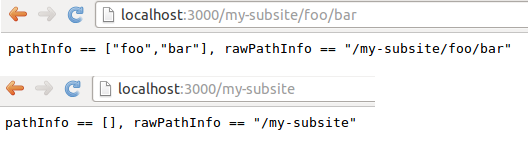
\includegraphics[width=0.9\textwidth]{17a-subsite-path-info.png}
  \caption{Информация о маршруте в подсайте}
\end{figure}

И, наконец, не все запросы будут содержать корректные пути. В этих случаях мы
хотим возвращать ответ <<404 Not Found>>.
\begin{lstlisting}
            _ -> yesodRunner (notFound >> return ()) env Nothing req
\end{lstlisting}
            
\subsection{Полный код}
Ниже представлен весь код примера, использующий подход без Template Haskell.

\includecode{17a/no-th-example.hs}

\subsection{Выводы}
Yesod даёт разработчику абстрагироваться от некоторой части черновой работы.
Большая часть которой~--- это шаблонный код, который вы будете рады
проигнорировать. Но понимание того, что конкретно происходит внутри, может
существенно расширить ваши возможности. К этому моменту, надеемся, вы должны
быть в состоянии, с помощью документации, написать сайт, не используя код,
генерируемый с помощью Template Haskell. Хотя я и не рекомендую это~--- я
думаю, что использовании генерируемого кода проще и безопаснее.

Одно особое преимущество понимания этого материала~--- в\emph{и}дение места
Yesod в мире WAI. Оно упрощает рассмотрение того, как Yesod будет
взаимодействовать с компонентом промежуточного уровня (middleware) WAI, или как
включить код из другого WAI фреймворка в Yesod (или наоборот!).
